\documentclass[10pt]{article} 
\usepackage{geometry, hyperref, booktabs, tikz}
\geometry{tmargin=1in, bmargin=1in, lmargin=2.5in, rmargin = 1in}  
\usepackage[dvipsnames]{xcolor}

\title{\textbf{U.S. Congress}\\\textit{Getting Re-elected}}
\author{Nathan Barron}
\date{Fall 2024}

\begin{document}
\maketitle
\tableofcontents
\vspace{.25in}
\hrule
\vspace{.25in}

\section{\textit{Constituencies}}

Richard Fenno identified four constituencies toward which the MC must be responsive: the geographic, general, primary, and personal constituencies. The geographic constituency is comprised of all persons within the boundaries of the Congressional district, whether they are voters or not. The general constituency (or supporters) is comprised of those voters who do or might vote for the MC. The primary constituency (or loyalists) are those who are engaged with the campaign, not only voting for the MC but also fundraising, campaigning, etc. The personal constituency (intimates) are those who are close to the MC (friends, family, acquaintances, etc.). The personal constituents need not be residents of the geographic constituency. 

\begin{figure}[h]
\centering
    \resizebox{0.4\textwidth}{!}{
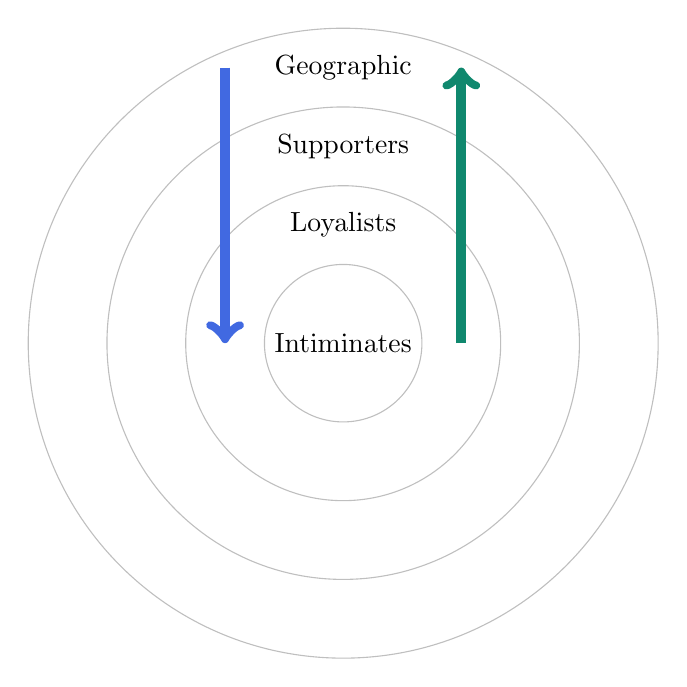
\begin{tikzpicture}
    % Draw the circles
    \draw[lightgray] (0,0) circle (1cm);
    \draw[lightgray] (0,0) circle (2cm);
    \draw[lightgray] (0,0) circle (3cm);
    \draw[lightgray] (0,0) circle (4cm);
    
    % Add the labels
    \node at (0, 0) {Intiminates};
    \node at (0, 1.5) {Loyalists};
    \node at (0, 2.5) {Supporters};
    \node at (0, 3.5) {Geographic};

    \draw[RoyalBlue,line width=1.25mm,->] (-1.5, 3.5) -- (-1.5,0) ;
    \draw[PineGreen,line width=1.25mm,->] (1.5, 0) -- (1.5, 3.5);
\end{tikzpicture}
    }
    \caption{\textbf{Graph representation of Fenno's Constituencies.} The MC's relationships and responsibilities differ with regard to how ``core" they are. The closer to the center, the more responsive the MC will be to that constituencies' needs. The further from the center, the fewer resources that constituency has to offer the MC.}
\end{figure}

\section{Election Trends}

\subsection{Primary elections}

\begin{itemize}
    \item MCs strive to prevent primary challengers (less differential, general election positioning)
    \item A well-tailored home style, fundraising, taking favorable actions in Congress, etc., can all prevent primary challenges
    \item When facing quality challengers, MCs tend to stick to party voting\footnote{Meyer, C. B. (2021). Getting ``Primaried” in the Senate: Primary Challengers and the Roll-Call Voting Behavior of Sitting senators. Congress \& the Presidency, 49(2), 230–251. https://doi.org/10.1080/07343469.2021.1922541}
    \item MCs also generally need to keep the party (and/or its factions) happy in order to prevent increased outside spending to finance quality challengers
    \item It is uncommon for incumbents to lose a primary: average of 5 incumbents per non-redistricting cycle since 2010; 13 in 2012 and 16 in 2022 (redistricting)
    \item Some recent incumbent losses in the House: Carolyn Maloney (Nadler 2022); Liz Cheney (Hageman 2022); Madison Cawthorn (Edwards 2022); Scott Tipton (Boebert 2020); Steve King (Feenstra 2020); Joe Crowley (Ocasio-Cortez 2018); Eric Cantor (Brat 2014); Silvestre Reyes (O'Rourke 2012)
    \item Successful primary challengers are rare in the Senate. The two most recent ``close calls" were in MA (2020 -- Markey \& Kennedy, 55-45) and AR (2010 -- Lincoln \& Halter, 52-48). 
    \item Last successful challenges were in 2014 (IN -- Lugar \% Mourdook, 39-61), 2010 (AK -- Murkowski \& Miller, 49-51; UT -- Bennett \& Lee, 49-51), and 2006 (CT -- Lieberman \& Lamont, 48-52).
\end{itemize}

\subsection{General elections}

\begin{itemize}
    \item Only 24 House races are considered to be a ``toss-up"\footnote{https://www.cookpolitical.com/ratings/house-race-ratings}, while only 43 House races were rated to be between D+3 and R+3 on the Cook Political PVI rating\footnote{https://www.cookpolitical.com/cook-pvi/2022-partisan-voting-index/introducing-2022-cook-partisan-voting-index}, down nearly 50\% since 2000; Most of the ``safe" seats belong to Republicans (205, as opposed to 185 for Democrats)
    \item 2 Senate races (MI and OH) are considered to be a ``toss-up", with 2 other seats (MT and WV) likely to be Republican flips
    \item Senate races can be more susceptible to national partisan trends due to larger constituencies, turnover due to ``promotion," Senator's behavior during term (more likely to engage in position-taking, less likely to be as visible to constituents as House members, etc.), etc.
    \item 9 House members lost their seat in the 2022 general election (1 redistricting)
    \item No Senators lost their seat in 2022; 5 Senators lost their seat in the 2022 general election (2 special elections); 5 Senators lost seats in 2018; 2 in 2016; 5 in 2014;  2 in 2012
\end{itemize}

\end{document}
